The third prototype built and the first thought to be the final version of the TRITIUM detector module was TRITIUM-Aveiro 0, shown in Figure \ref{fig:TritiumAveiro0}, which was designed and built in the workshop of the University of Aveiro. 

\begin{figure}[h]
\centering
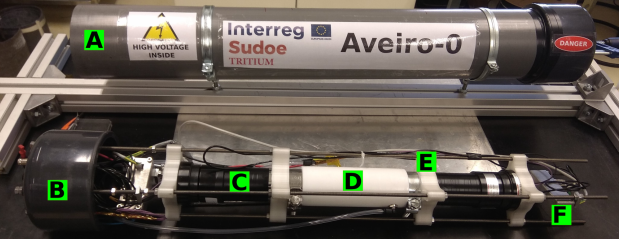
\includegraphics[scale=0.4]{5Prototypes/53FinalPrototypes/531TritiumAveiro/GeneralViewOfAveiroPrototype.png}
\caption{TRITIUM-Aveiro prototype.\label{fig:TritiumAveiro0}}
\end{figure}


It consists of a teflon vessel (D of Figure \ref{fig:TritiumAveiro0}), shown in Figure \ref{fig:TeflonStructureFibersTritiumAveiro0}, which has an internal cylindrical hole the diameter and length of which are $43~\mm$ and $18~\cm$ respectively. 

\begin{figure}[h]
\centering
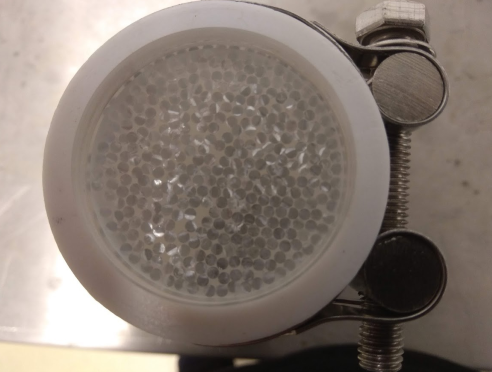
\includegraphics[scale=0.4]{5Prototypes/53FinalPrototypes/531TritiumAveiro/TeflonVessel_Fibers.png}
\caption{Teflon structure and fiber bundle used in TRITIUM-Aveiro 0 prototype.\label{fig:TeflonStructureFibersTritiumAveiro0}}
\end{figure}

This vessel contains $360$ no-clad scintillating fibers with a length of $180~\mm$. The model of the used fibers is BCF-10 from Saint-Gobain company \cite{DataSheetBCF10Fiber}, which have practically the same characteristics than the others used up to now (BCF-12 fibers) and their most important difference is their diameter, which is the double, $2~\mm$.

A larger diameter could be interesting because it facilitates the flow of water around the fibers, reducing the problems related to surface tension and ensuring that the entire active volume of the fibers is used for tritium detection. In addition, it increase the resistance of the fibers, which is very important since the water is flow around them. However, it could be detrimental since this worsens the signal-to-background ratio. The detector active volume for $2~\mm$ fibers in the same space is smaller, producing a smaller tritium signal and the part of the fibers where no tritium events reach (they only contribute to the background) is larger, producing a larger background. As a result, a worse signal-to-background ratio will be achieved.

In order to quantify the importance of the fiber diameter effect, the measurements were compared with similar measurements performed with TRITIUM-IFIC 2 prototype, shown in section \ref{subsec:TritiumIFIC2}, based on a similar configuration with $1~\mm$ fibers (BCF-12 model).

The amount of fibers used in TRITIUM-Aveiro 0 prototype is the maximum which allows the water to flow around the fibers. It has to be taken into account that it was not possible to use a structure to fix the fibers due to the large amount of them, so they will remain free inside of the teflon vessel. 

These fibers were cut with the fiber cutting device developed by TRITIUM but they were neither polished nor cleaned. The reason for this is that the automatic polishing machine was not yet developed and it was not feasible to polish 360 fibers by hand. In fact, the automatic polishing machine was motivated by the amount of fibers used in the last prototypes.

To ensure the radiosecurity of this prototype, the teflon vessel is totally closed and  a water inlet/outlet were installed in it to allow a constant water flux through it. Two PMMA windows was used to read the fibers, whose thick is $10~\mm$, which was located at both ends of the fiber bundle and two clamps are used to press the Teflon walls against the PMMA windows to ensure the water tightness of the prototype. PMMA was chosen for its optical properties, especially its transmission coefficient, which is more than $95\%$ for the working wavelength.

Two PMTs (C of Figure \ref{fig:TritiumAveiro0}) are used to read this prototype in time coincidence, which are powered at $-1500~\volt$, at which the quantum efficiency is $26\%$. They are fixed to both fiber bundle ends of the prototype using two pieces (E of Figure \ref{fig:TritiumAveiro0}) which was designed and built with a 3D printer. Both PMTs are optically coupled to the PMMA windows using optical grease \cite{OpticalGrease}.

The PMTs used are the model R2154-02 2" from Hamamatsu company \cite{DataSheetPMTsAveiro}, whose characteristics, specially its gain and efficiency, are quite similar to the PMTs used in the other prototypes.

All these different parts, together with the electronic system (F of Figure \ref{fig:TritiumAveiro0}), is arranged in a structure, shown in Figure \ref{fig:TritiumAveiro0}, which is based on several nuts located on four long stainless-steel screws. This screws are fixed to an external PVC structure, A and B of Figure \ref{fig:TritiumAveiro0}, which is used to protect the prototype from physical damage and provide a light-tight operation environment. This PVC structure is equiped with several high voltage power, low voltage power and signals feed-through connectors.

Only one prototype was built, which was designed to be installed in the Arrocampo dam and an electronic chain, based on several PCBs, was specially designed, developed, built and tested to process and analyze the signals of this system, shown in appendix \ref{App:ElectronicSystemAveiro}.

Two interfaces were developed, one to control the power supply to the PMTs, shown in Figure \ref{subfig:GUIHV}, and the other to control the different options of the electronic reading chain, such as thresholds and measured counts, shown in Figure \ref{subfig:GUIcounts}.

\begin{figure}
\centering
    \begin{subfigure}[b]{0.65\textwidth}
    \centering
    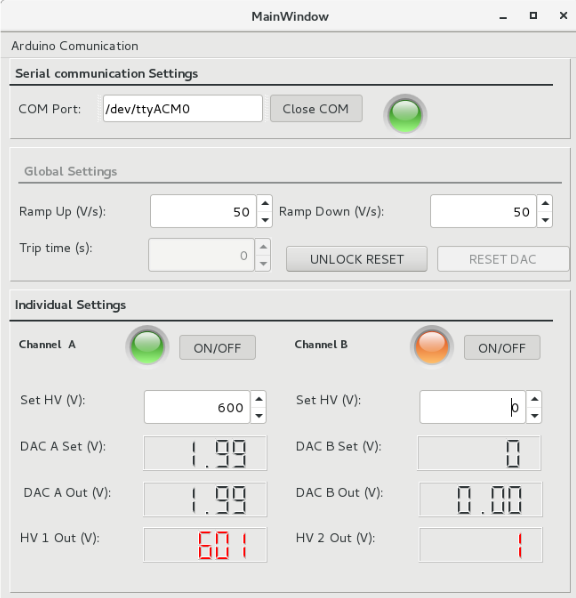
\includegraphics[width=\textwidth]{5Prototypes/53FinalPrototypes/531TritiumAveiro/GUIHVBoard.png}  
    \caption{Graphical user interface to manage the power supply voltage of PMTs.\label{subfig:GUIHV}}
    \end{subfigure}
    \hfill
    \begin{subfigure}[b]{0.8\textwidth}
    \centering
    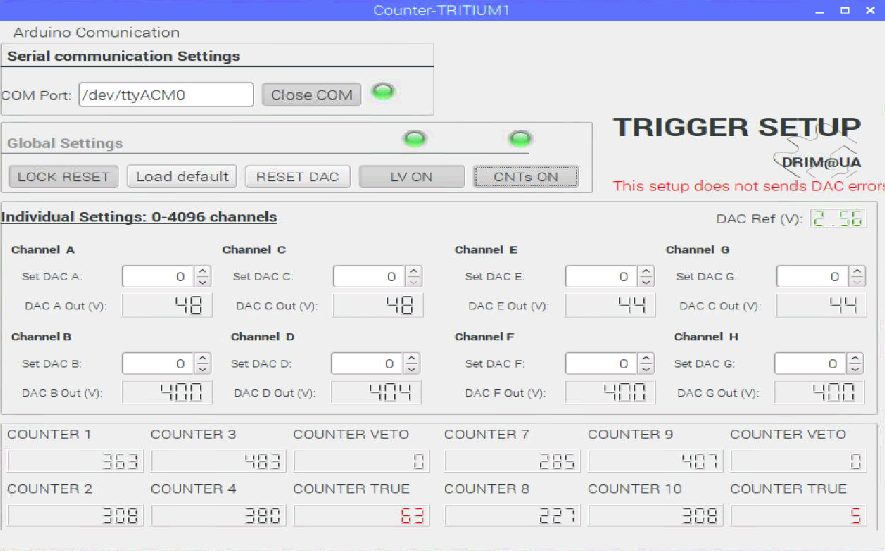
\includegraphics[width=\textwidth]{5Prototypes/53FinalPrototypes/531TritiumAveiro/CounterGUI.png}  
    \caption{Graphical user interface used to manage the counter system.\label{subfig:GUIcounts}}
    \end{subfigure}
 \caption{Graphical User Interface developed to control the TRITIUM-Aveiro prototype.}
 \label{fig:GUITRITIUMAveiro}
\end{figure}

First some measurements were taken in the laboratory, which were used to characterize the detector. For this task it was firstly filled with ultra-pure water, which was used to measure the background of the detector, and then, with a radioactive liquid tritium solution with an activity of $30~\kilo\becquerel/\liter$, which were used the mesure the efficiency and the low detection level, LDL, of the prototype. The volume of ultrapure water and tritium solution used in TRITIUM-Aveiro 0 prototype is $58~\milli\liter$. Later, it was installed in the arrocampo dam to test its functionality and to begin with the tritium level monitoring. The laboratory and Arrocampo measurements, both, are shown in section \ref{subsec:ResultsTritiumAveiro} and \ref{sec:ResultsArrocampo} respectively, where they are discussed and compared with the measurements of the previous prototypes.